\begin{frame}\frametitle{Background}
Main idea: train a netowork on a "fake task" then use the weights as embedding. \bigskip
\begin{itemize}
\item The fake task:
\begin{itemize}
\item Given a word $w$ guess the context words. 
\end{itemize}
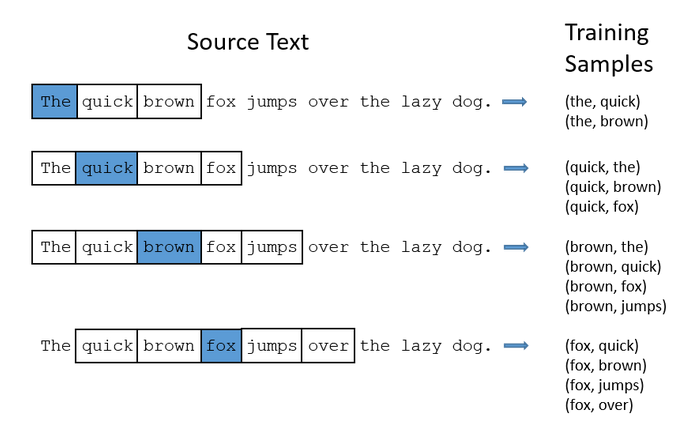
\includegraphics[scale=0.37]{images/context_pairs.pdf}
\end{itemize}
\end{frame}

\begin{frame}\frametitle{Background}\framesubtitle{Network achitecture}
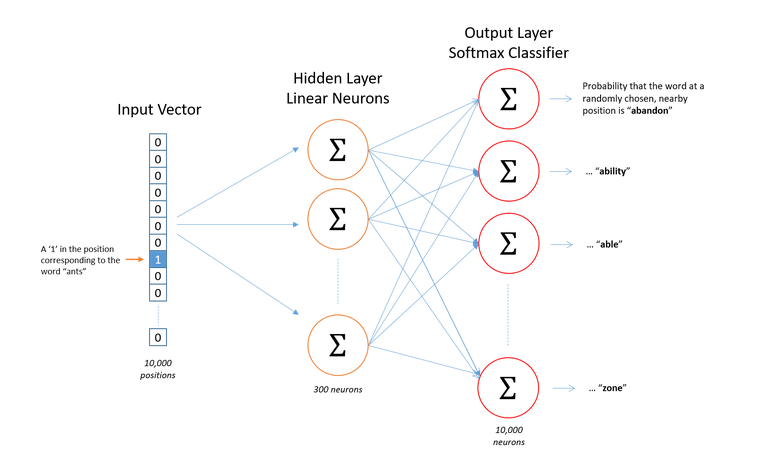
\includegraphics[scale=0.37]{images/ntw_architecture.png}
(Source: http://mccormickml.com/2016/04/19/word2vec-tutorial-the-skip-gram-model/) 
\end{frame}

\begin{frame}\frametitle{Background}\framesubtitle{Softmax}
\begin{Large}
It's unsuitable to compute the softmax
\end{Large}
   \begin{equation}
   p(w_{t+j}|w_t)=  \frac{exp( \tilde{v}_{w_{t+j}}^Tv_{w_t})}{\sum_{w=1}^T exp(\tilde{v}_w^Tv_{ w_t})}
   \end{equation}
   
   For each pair we have to go over the whole training corpus. (Billions of word in practice) 
   What can we do? 
\end{frame}

\begin{frame}\frametitle{Background}\framesubtitle{Negative Sampling}
Idea cam from NCE introduced by .. 
distinguish data from noise reduce problem to a logistic regression. 

we do not care about logistic regression only about good vector representation
guess k random samples 
  \begin{align*}
p(c|w) &= p(y=1|c,w) + \prod_{k\in K} p(y=0|k,c) 
\\&= log(\sigma(v_c v_w ) + \sum_{k\in K} \sigma(log(-v_w v_k )) &&\text{$ where, \sigma = \frac{1}{1+e^{-x}}$}
\end{align*}
\end{frame}